\chapter{COMPOSIÇÃO DA OBRA}

Dentre os componentes da instalação interativa proposta neste trabalho, podemos destacar a interface, representada pelo sensor Microsoft Kinect, que parece invisível dado que o interator precisa apenas estar com o seu corpo presente no espaço para que a obra se materialize; o gerenciamento digital que é feito através de um computador e da utilização de \textit{Processing} para execução e manutenção do programa; e, por fim, o dispositivo de saída de dados, aqui reprensentado por uma composição entre a malha de LEDs e o Arduino, traduzindo informação em luz.

Devido ao recurso de capturar objetos e movimentos no espaço, optou-se pelo uso do sensor Microsoft Kinect que, conectado a um computador, é responsável por captar a área onde os espectadores se encontram. Integrando-o a uma placa Arduino é possível controlar uma série de LEDs, dispostos em uma grade pendente ao teto. Cada LED possui cabos de fibra ótica \textit{side light} (com emissão de luz lateral) conectados à ele que se iluminam conforme os espectadores caminham sob a grade. Na figura \ref{fig:esquema} podemos ver um esquema de montagem da obra, sendo que, o sensor Kinect fica preso junto ao teto, a grade com os LEDs se encontra abaixo, a pouco mais de um metro de distância, deixando espaço suficiente para os espectadores transitarem.

\begin{figure}[H]
    \centering
    \caption{Esquema de montagem da obra.}
	\vspace*{0,2cm}
    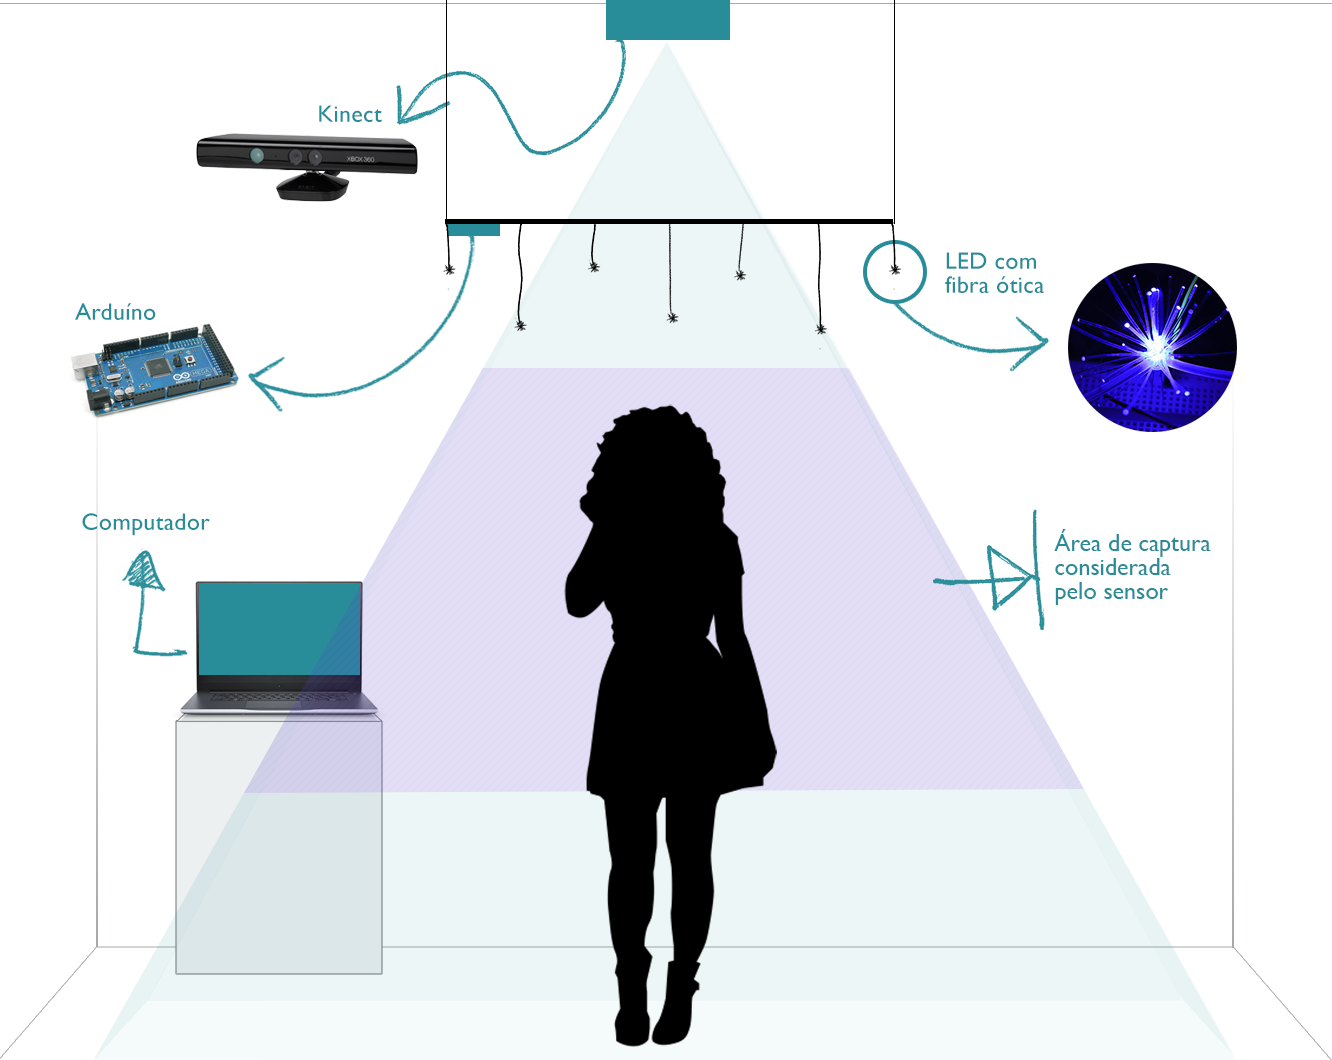
\includegraphics[width=0.8\textwidth]{./04-figuras/esquema}
    \label{fig:esquema}
\end{figure}
\vspace*{-0,9cm}
{\raggedright \fonte{Elaborada pela autora}}\\

A seguir veremos um detalhamento dos componentes e nos aprofundaremos sobre o papel de cada um deles neste trabalho. 

\section{MICROSOFT KINECT}

O sensor Kinect é um dispositivo lançado em 4 de Novembro de 2010 como um acessório do console Xbox 360 da Microsoft. Orientado, principalmente, a indústria de jogos, foi criado para servir como uma forma de interação entre o utilizador e o console Xbox 360 através de gestos e comandos de voz. De acordo com a \citeonline{microsoft}, em sua primeira versão, é capaz de capturar imagens com 640x480 pixels a 30 fps. O aparelho é formado por um sensor de profundidade, uma câmera RGB, um acelerómetro, um motor e uma série de 4 microfones. Na figura \ref{fig:kinect_componentes} podemos ver a posição de cada um destes componentes no dispositivo.

\begin{figure}[H]
    \centering
    \caption{Componentes do sensor Kinect}
	\vspace*{0,2cm}
    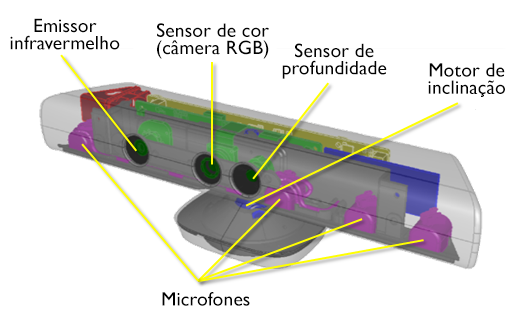
\includegraphics[width=0.8\textwidth]{./04-figuras/kinect_componentes}
    \label{fig:kinect_componentes}
\end{figure}
\vspace*{-0,9cm}
{\raggedright \fonte{\citeonline{microsoft}}}\\

Dentre seus componentes, o que mais nos interessa no contexto deste trabalho, é o sensor de profundidade. \citeonline{ashley} afirmam que a produção de dados tridimensionais é a principal função do Kinect. Ele difere de qualquer outro dispositivo de entrada justamente porque provê uma terceira dimensão e, para tanto, se utiliza de um emissor e uma câmera de infravermelho. Segundo \citeonline{lucero} o emissor de infravermelhos projeta um padrão estruturado de luz infravermelha, enquanto a câmera lê esses raios e interpreta a deformação da projeção, convertendo essa informação em valores de profundidade e, consequentemente, medindo a distância entre o objeto e o sensor. De acordo com \citeonline{correia} estas medidas baseiam-se em triangulação tendo em conta o emissor, a câmera e as posições dos pixels no cenário. A profundidade é codificada numa escala de cinzas. Quanto mais escuro o pixel, mais próximo do sensor está esse ponto no espaço. Sendo que, pixels pretos indicam que não existe informação de profundidade. Isto ocorre no caso dos pontos estarem muito longe, impossibilitando a sua captura, no caso de estarem numa área onde não haja pontos do emissor de infravermelhos, no caso de o objeto refletir mal a luz infravermelha ou, finalmente, no caso de os pontos estarem muito próximos do sensor, uma vez que o campo de visão do Kinect é limitado em cerca de 80 centímetros a 4 metros.

Considerando as limitações do sensor Kinect, a que mais impactou este projeto é causada pela própria natureza da luz projetada pelo sensor. A luz emitida pelo projetor de infravermelho, ao se deparar com um objeto, gera uma sombra em outro que esteja numa distância maior. Segundo \citeonline{lucero} o resultado é que não se pode determinar a profundidade em zonas afetadas por estas sombras, como pode ser visto na figura \ref{fig:kinect_sombras}. Dessa forma, estas sombras criam zonas negras na imagem de profundidade, ou seja, pixels com valor zero. O impacto gerado aqui é devido à malha de LEDs se encontrar entre o sensor Kinect e o espectador. A malha projeta uma sombra, criando pontos onde o espectador pode não ser percebido.  Mais detalhes sobre essa questão serão vistos na seção \ref{sec:malha} \nameref{sec:malha}.

\begin{figure}[H]
    \centering
    \caption{Efeito das sombras no sensor Kinect}
	\vspace*{0,2cm}
    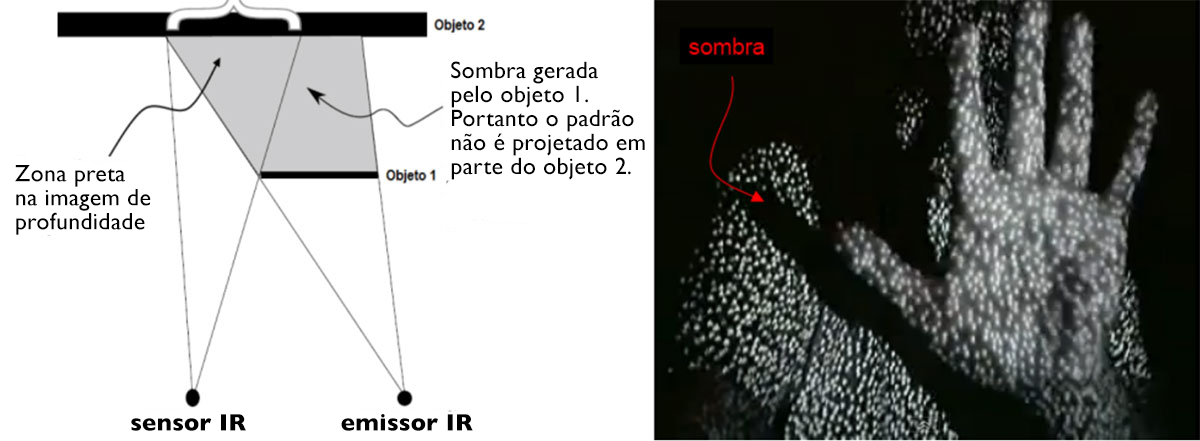
\includegraphics[width=0.8\textwidth]{./04-figuras/kinect_sombras}
    \label{fig:kinect_sombras}
\end{figure}
\vspace*{-0,9cm}
{\raggedright \fonte{\citeonline{lucero}}}\\


O Microsoft Kinect atua como interface da instalação interativa proposta neste trabalho, sendo utilizado como fonte de entrada (\textit{input}) de dados para mapear o ambiente tridimensional. A figura \ref{fig:kinect_exemplo} mostra um exemplo de imagem criada a partir dos dados capturados pelo sensor. Cada ponto branco apresentado na figura representa um LED aceso na estrutura física, enquanto a área em preto demarca os intervalos entre os mesmos. Não há distinção, na imagem, entre estes intervalos e os LEDs apagados. 

\begin{figure}[H]
    \centering
    \caption{Imagem gerada a partir  das informações capturadas  pelo sensor Kinect.}
	\vspace*{0,2cm}
    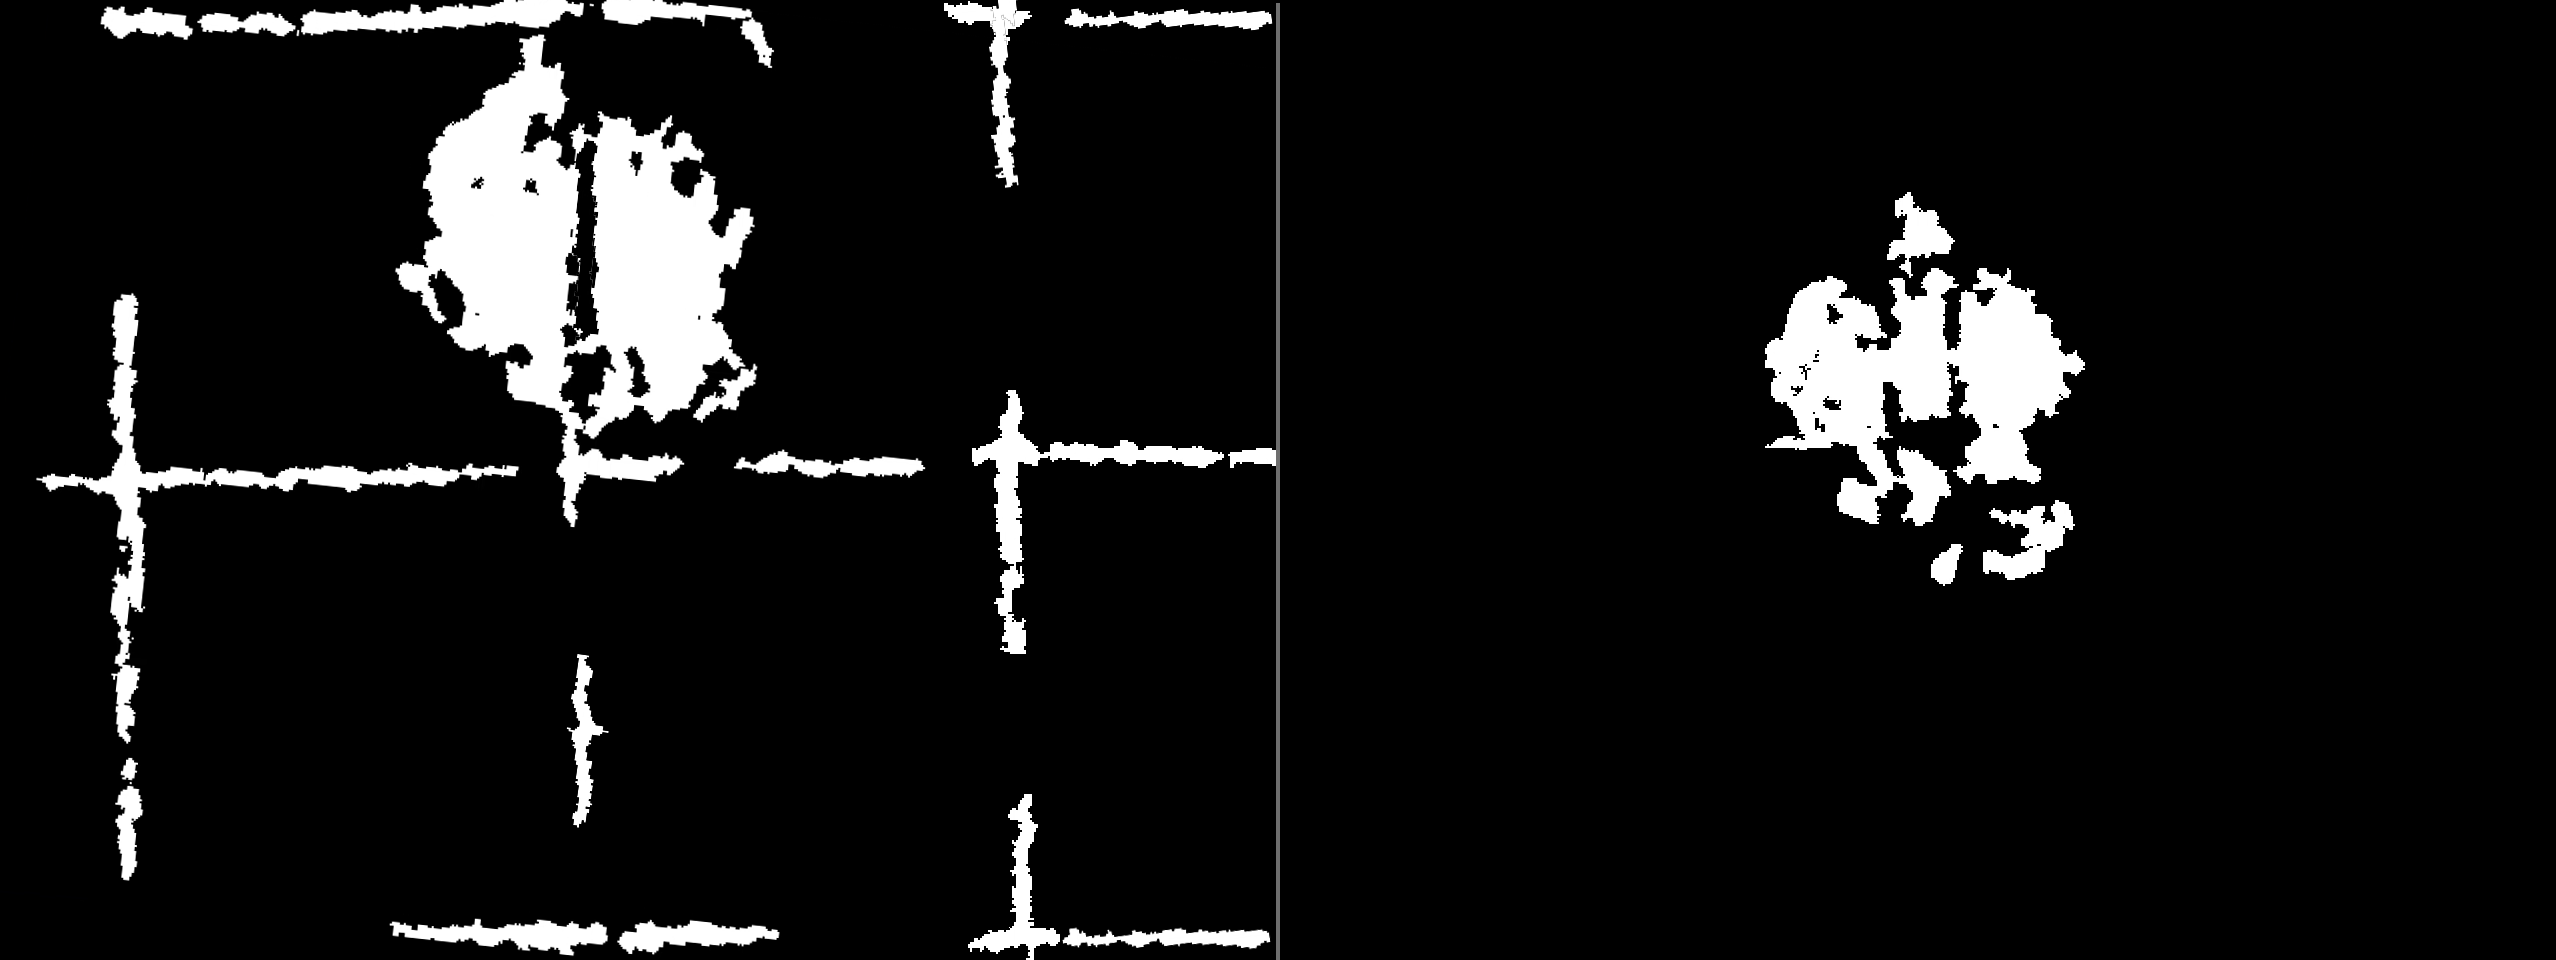
\includegraphics[width=0.8\textwidth]{./04-figuras/kinect_exemplo}
    \label{fig:kinect_exemplo}
\end{figure}
\vspace*{-0,9cm}
{\raggedright \fonte{Captura de tela de imagem gerada pelo sensor Kinect}}\\


\section{PROCESSING}

De acordo com \citeonline[p. 115]{santos} Processing é a primeira ferramenta criada para artistas por artistas e o seu desenvolvimento foi iniciado no MIT Media Lab por dois estudantes de graduação: Casey Reas e Benjamin Fry. Segundo informações contidas no site oficial do projeto \citeonline{processing} é uma plataforma e uma linguagem de programação de código aberto (\textit{open source}) para prototipação de \textit{software} dentro do contexto das artes visuais. Disponível desde 2001, a Processing promoveu a alfabetização em \textit{software} dentro das artes visuais e a alfabetização visual dentro da tecnologia. Há dezenas de milhares de estudantes, artistas, designers, pesquisadores e amadores que usam Processing para aprender e criar protótipos.

O gerencimento digital da obra é realizado através de um computador que executa um programa escrito em Processing, interpretando as informações fornecidas pelo Kinect e gerando uma imagem bidimensional que, mais tarde, é transferiada para o Arduino e reproduzida na estrutura de LEDs. 


\section{ARDUINO}

Para compreender o que é e para que serve o Arduino, podemos analisar a descrição presente no \textit{site} oficial do projeto:

\begin{citacao}
Arduino é uma plataforma de prototipagem eletrônica de \textit{hardware} livre e de placa única. O objetivo do projeto é criar ferramentas que são acessíveis, com baixo custo, flexíveis e fáceis de usar. Placas arduíno são capazes de ler uma entrada como a luz em um sensor, um dedo pressionando um botão ou uma mensagem do Twitter e transformá-la em uma saída como ativar um motor, ligar um LED ou publicar alguma coisa na internet, por exemplo. É possível dizer à placa o que fazer enviando uma série de instruções ao microcontrolador. Para isso é necessário utilizar a linguagem de programação do Arduino (baseada em Wiring) e o seu software (IDE - \textit{Integrated Development Environment} ou Ambiente de Desenvolvimento Integrado), baseada em Processing \cite{arduino}. 
\end{citacao}

Neste trabalho o Arduino foi utilizado para controlar os circuitos da malha de LEDs (saída ou \textit{output}) recebendo as informações mapeadas pelo sensor Kinect (entrada ou \textit{input}). Cada LED precisa ser controlado individualmente, por isso, à princípio, optou-se pela utilização do Arduino Mega que possui 54 entradas/saídas digitais, sendo a placa disponível com o maior número de entradas/saídas. Ainda se encontra em definição a maneira como o trabalho será escalado para atingir as dimensões propostas na próxima sessão deste capítulo. Considera-se a possibilidade de utilizar mais de uma placa Arduino, circuitos multiplexadores - que permitem que em uma única porta sejam conectados mais de um LED -, ou ainda, a construção de uma placa sob medida.

\section{MALHA DE LEDS}

A malha delimita o espaço da instalação. Será construída uma grade de LEDs formada por quatro módulos de 120 x 80 cm, constituindo uma área total de 2,4 x 1,6 metros onde o espectador pode interagir com a obra. As grades possuem intercesções a cada 20 centímetros, em ambos os sentidos, e cada intersecção possui um LED preso à ela. Na figura \ref{fig:malha} podemos ver um esquema dessa grade, sendo que, são apresentados exemplos de apenas 3 LEDs para não poluir o esquema.

\begin{figure}[H]
    \centering
    \caption{Esquema da malha de LEDs}
	\vspace*{0,2cm}
    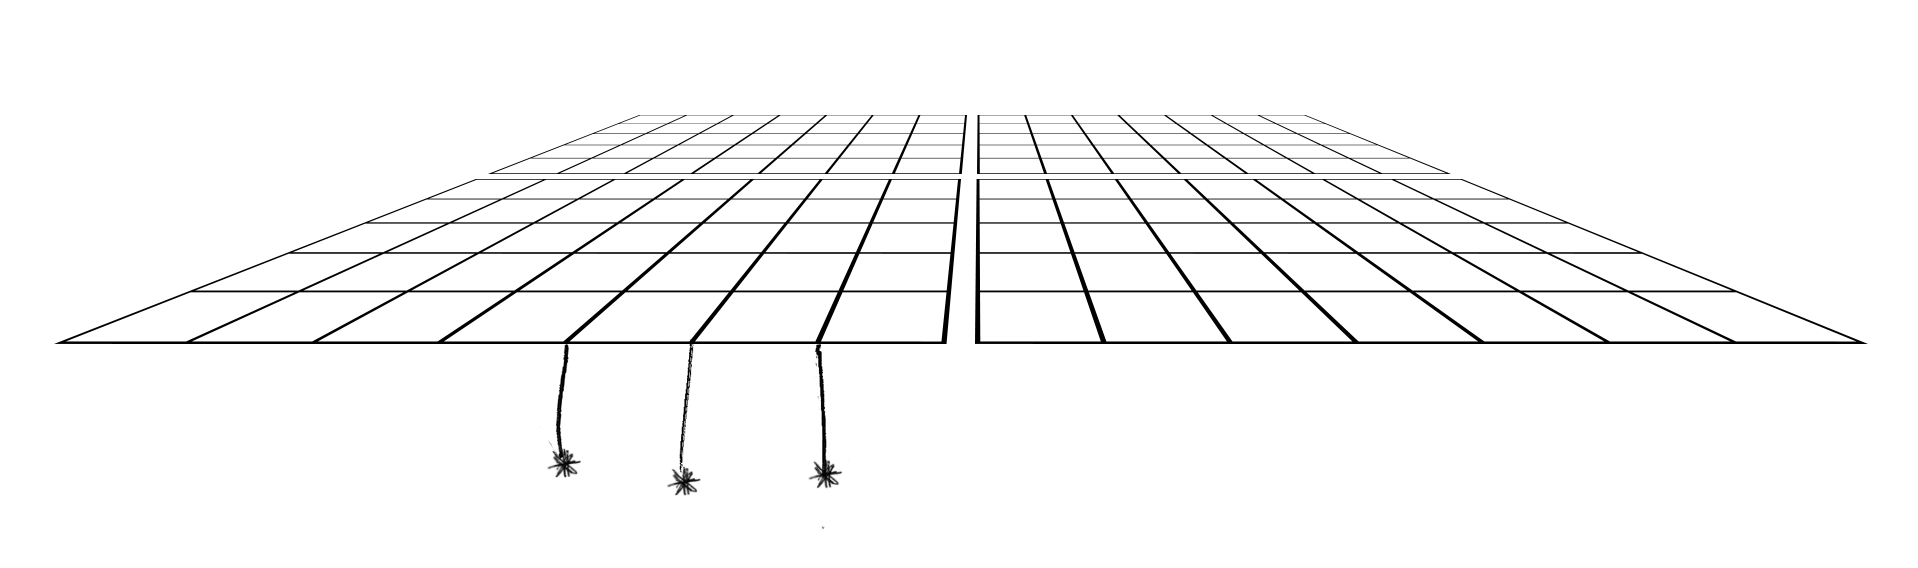
\includegraphics[width=0.8\textwidth]{./04-figuras/malha}
    \label{fig:malha}
\end{figure}
\vspace*{-0,9cm}
{\raggedright \fonte{Elaborada pela autora}}\\

Cada LED representa um ponto da imagem processada pelo sistema computacional e conta com fios de fibra ótica, com emissão de luz lateral, de várias espessuras presos em sua extremidade. Quando o LED acender, a partir da interação com o usuário, a luz será transmitida pela fibra ótica, gerando se transformando em vários pontos iluminados. Na figura \ref{fig:led_fibra_otica} podemos ver o exemplo de um desses LEDs, sendo que, no primeiro quadro o LED é exbido apagado, no segundo aceso em ambiente com alta luminosidade e, por fim, no terceiro quadro, aceso em ambiente com baixa luminosidade. 

\begin{figure}[H]
    \centering
    \caption{LED com fibra ótica em diferentes condições de luminosidade}
	\vspace*{0,2cm}
    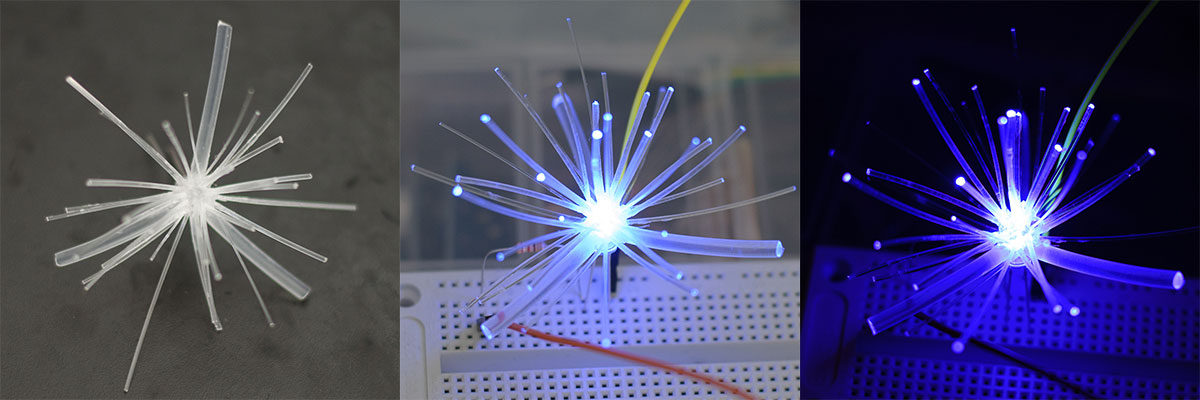
\includegraphics[width=0.8\textwidth]{./04-figuras/led_fibra_otica}
    \label{fig:led_fibra_otica}
\end{figure}
\vspace*{-0,9cm}
{\raggedright \fonte{Elaborada pela autora}}\\


\section{PROTÓTIPO}

Para validar o projeto foi construído um protótipo que conta com o Microsoft Kinect, um computador, um Arduino e 5 LEDs conectados à ele conforme pode ser visto na figura \ref{fig:prototipo}. Através da utilização de duas bibliotecas, \textit{Open Kinect for Processing} e Arduino (Firmata), foi possível construir um \textit{script} que controla os dispositivos de entrada e saída de forma integrada, causando assim o acender e apagar dos LEDs de acordo com a presença do espectador.

\begin{figure}[H]
    \centering
    \caption{Componentes do prótotipo}
	\vspace*{0,2cm}
    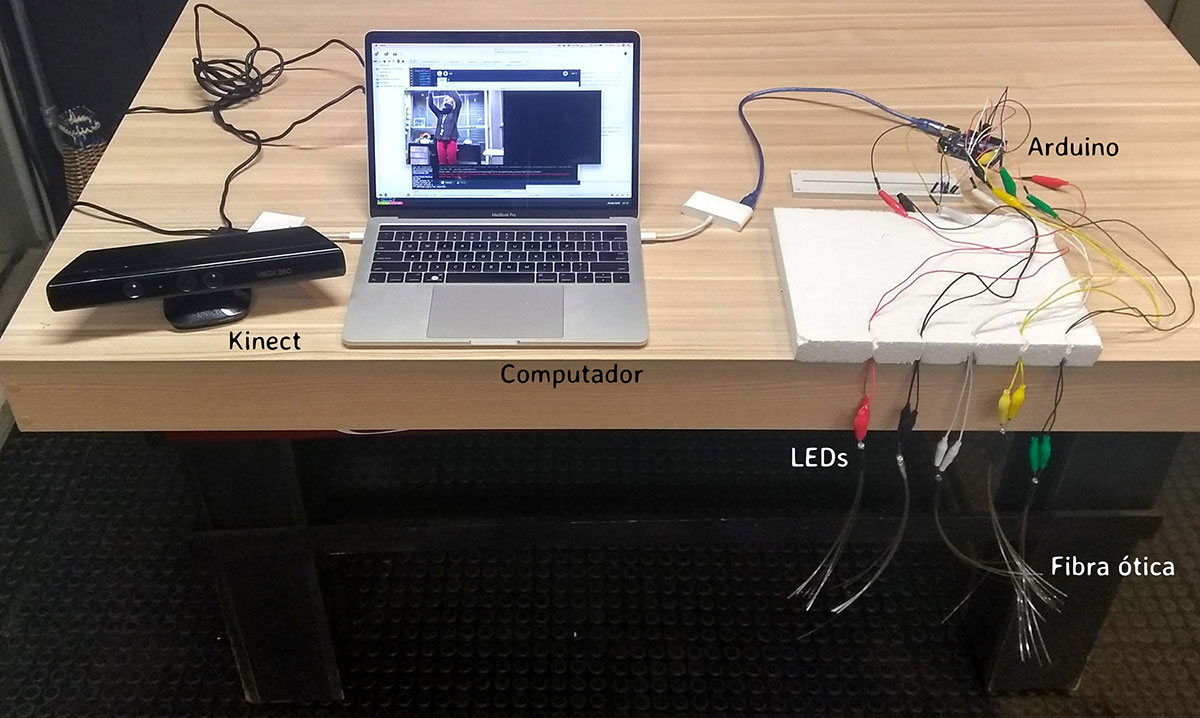
\includegraphics[width=0.8\textwidth]{./04-figuras/prototipo}
    \label{fig:prototipo}
\end{figure}
\vspace*{-0,9cm}
{\raggedright \fonte{Elaborada pela autora}}\\

Na figura \ref{fig:prototipo-escuro} podemos ver uma amostra do protótipo sendo executado em um ambiente com baixa luminosidade, o que reforça a escolha do cubo preto como sendo o melhor cenário para exibição desse trabalho.
 
\begin{figure}[H]
    \centering
    \caption{Protótipo em ambiente com baixa luminosidade}
	\vspace*{0,2cm}
    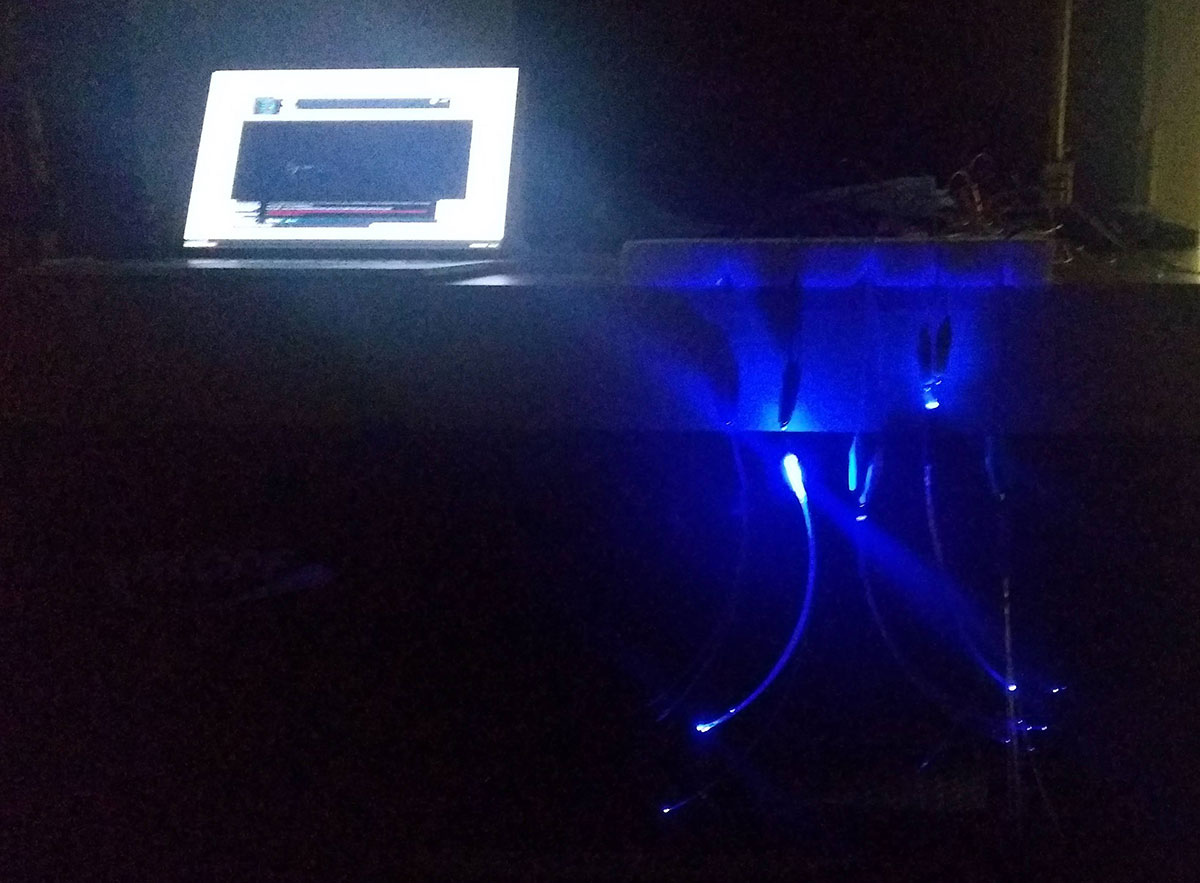
\includegraphics[width=0.8\textwidth]{./04-figuras/prototipo_escuro}
    \label{fig:prototipo-escuro}
\end{figure}
\vspace*{-0,9cm}
{\raggedright \fonte{Elaborada pela autora}}\\

   